This section presents the `Layer Method' for solving the cube. This algorithm is far from optimal, but is easy for beginners to learn. We shall start with the white face for this example; in general, one can start from any face.

\paragraph{Matters of notation} This section utilises standard Rubik's Cube notation to describe the solution. Consult Appendix ~\ref{app:notation} for information on this notation.

\subsection{Cross}
	This first step requires correctly placing any edge with white; this completes the `cross' on the white face and aligns the edges appropriately. This results in the configuration shown in \figref{topcross}.
\begin{figure}[h]
	\centering
	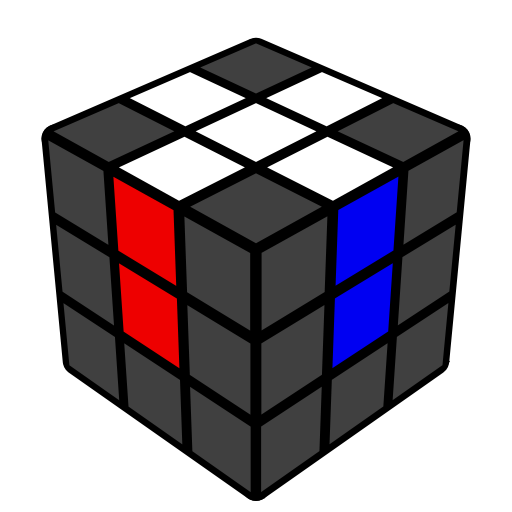
\includegraphics[width=0.3\textwidth]{topcross.png}
	\caption{Solved white cross}\label{fig:topcross}
\end{figure}

\begin{enumerate}
	\item \label{step:find} Find a white edge piece on the bottom layer.
	\item \label{step:align} Twist the bottom layer to align the piece you found with the corresponding non-white centre.
	\item Bring the piece to the top layer:\begin{enumerate}
		\item If the edge is already correctly aligned with the centre, twist it 180\degree , as seen in \figref{edgeup180}.
		\item Otherwise, twist it 90\degree to move it to the middle layer on a different face. Twist that new face to bring it back to the bottom layer. Then, go back to step~\ref{step:align}. This is shown in \figref{edgeup90}.
	\end{enumerate}
\begin{figure}[h]
	\centering
	\begin{subfigure}[b]{0.3\textwidth}
		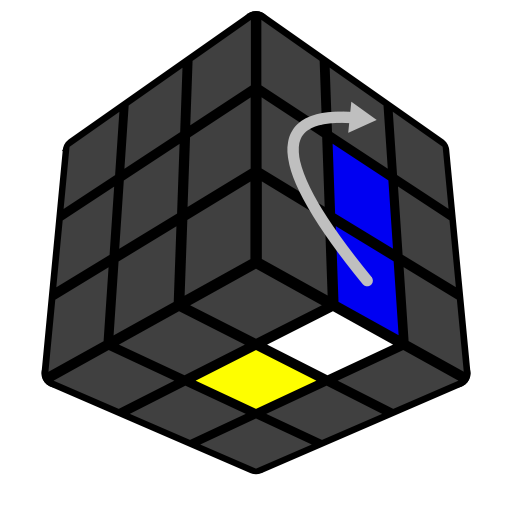
\includegraphics[width=\textwidth]{turn180.png}
		\caption{If aligned}{\label{fig:edgeup180}}
	\end{subfigure}
	\begin{subfigure}[b]{0.3\textwidth}
		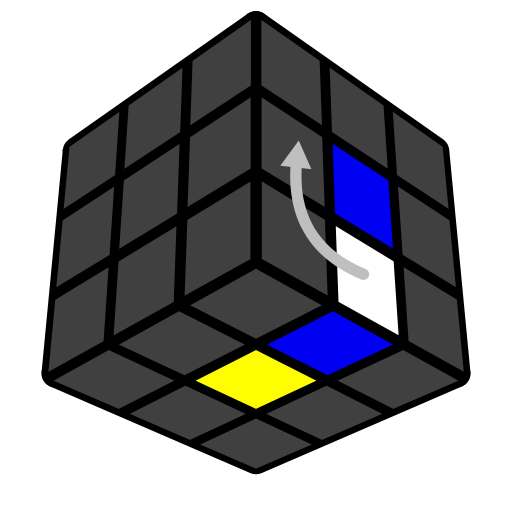
\includegraphics[width=\textwidth]{turn90.png}
		\caption{If not aligned}{\label{fig:edgeup90}}
	\end{subfigure}
	\caption{Bringing edges up}
\end{figure}
\newpage
	\item Repeat from step~\ref{step:find} until there are no more white edges on the bottom layer.
	\item Bring any white edges on the middle layer to the bottom layer by twisting 90\degree .
	\item Repeat from step~\ref{step:find} until there are no more white edges on the middle layer.
	\item Bring \emph{unsolved} white edges to the bottom layer by twisting 180\degree .
	\item Repeat from step~\ref{step:find} until the cross is complete.
\end{enumerate}



\subsection{Corners}
In this section, we correctly place corners. This completely solves the top layer as shown in \figref{toplayer}.
\begin{figure}[h]
	\centering
	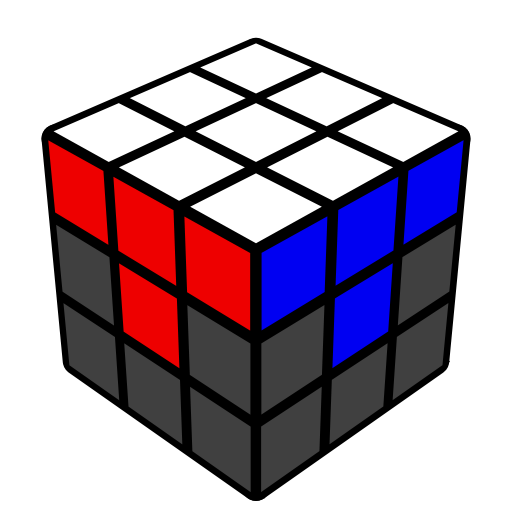
\includegraphics[width=0.3\textwidth]{toplayer.png}
	\caption{Solved top layer}\label{fig:toplayer}
\end{figure}
\begin{enumerate}
	\item Find an unsolved corner piece and bring it to the bottom layer.
	\item Twist the bottom layer to bring it underneath where it is supposed to go. It will then be in one of the configurations shown in \figref{confs}.
\begin{figure}[h]
	\centering
	\begin{subfigure}[b]{0.3\textwidth}
		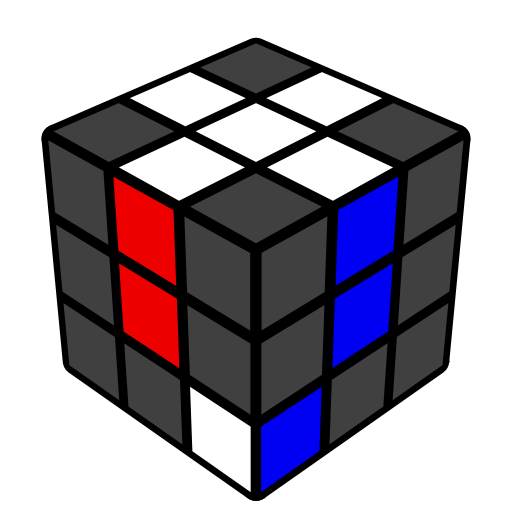
\includegraphics[width=\textwidth]{conf1.png}
	\end{subfigure}
	\begin{subfigure}[b]{0.3\textwidth}
		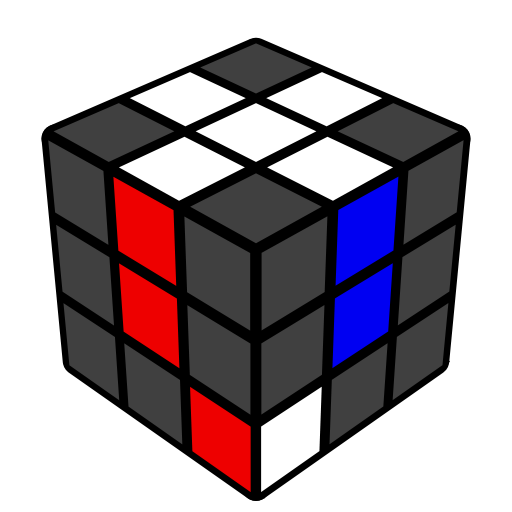
\includegraphics[width=\textwidth]{conf2.png}
	\end{subfigure}
	\begin{subfigure}[b]{0.3\textwidth}
		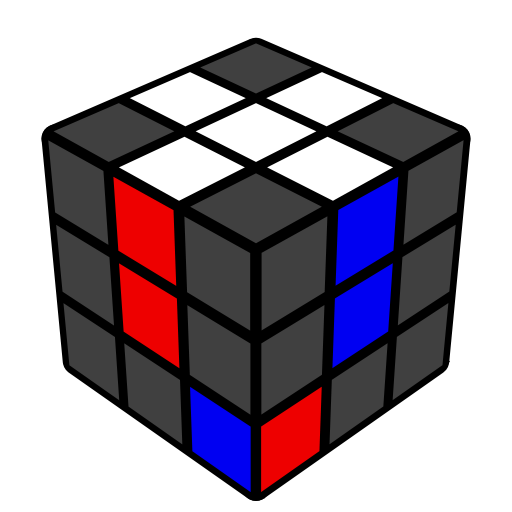
\includegraphics[width=\textwidth]{conf3.png}
	\end{subfigure}
	\caption{Possible configurations of the corner piece.}\label{fig:confs}
\end{figure}
	\item Hold the cube so that the corner appears at the bottom-right of the front face.
	\item Perform the algorithm \alg{R'D'RD} repeatedly until the corner is solved.
	\item Repeat from step 1 until all corners are solved.
\end{enumerate}

\subsection{Middle Layer}
This section solves the middle layer to arrive at \figref{midlayer}.
\begin{figure}[h]
	\centering
	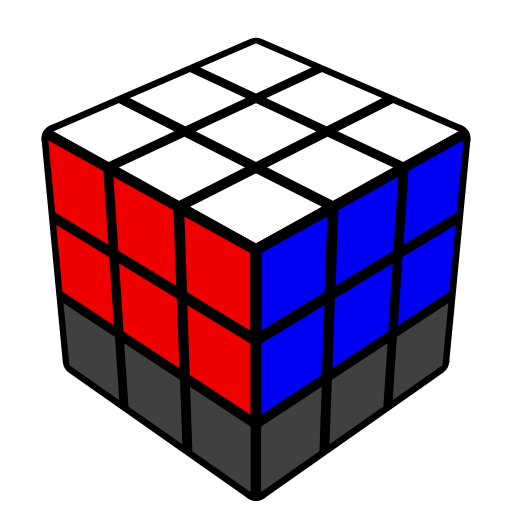
\includegraphics[width=0.3\textwidth]{midlayer.png}
	\caption{Solved middle layer}\label{fig:midlayer}
\end{figure}
\begin{enumerate}
	\item Flip the cube so that the white face is on the bottom. This allows you to observe the bottom (now top) layer easily.
	\item Find an edge on the new top layer that belongs in the middle layer.
	\item Align the side of that edge with the corresponding centre on the middle layer.
	\item The top face of the edge will be in one of the following configurations. Holding the edge in front of you, perform the appropriate algorithm:\begin{enumerate}
		\item Matches the left centre (as in \figref{midconf1}); do \alg{U'L'ULUFU'F'}.
		\item Matches the right centre (as in \figref{midconf2}); do \alg{URU'R'U'F'UF}.
	\end{enumerate}
\begin{figure}[h]
	\centering
	\begin{subfigure}[b]{0.3\textwidth}
		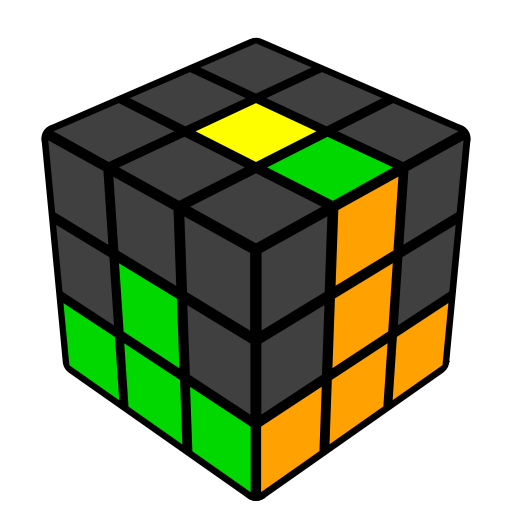
\includegraphics[width=\textwidth]{midconf1.png}
		\caption{Matches left}\label{fig:midconf1}
	\end{subfigure}
	\begin{subfigure}[b]{0.3\textwidth}
		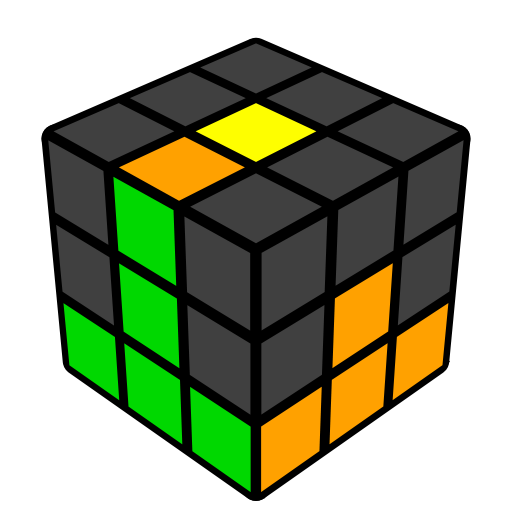
\includegraphics[width=\textwidth]{midconf2.png}
		\caption{Matches right}\label{fig:midconf2}
	\end{subfigure}
	\caption{Possible configurations of the middle edge.}
\end{figure}
	\item Repeat from step 1 until the middle layer is done.
	\item Flip the cube back to white on top.
\end{enumerate}


\subsection{Bottom Cross}
The general strategy for this stage is:\begin{enumerate}
	\item Make a (not necessarily aligned) cross, see \figref{fakecross}.
	\item `Fix' the cross, see \figref{realcross}.
\end{enumerate}
\begin{figure}[h]
	\centering
	\begin{subfigure}[b]{0.3\textwidth}
		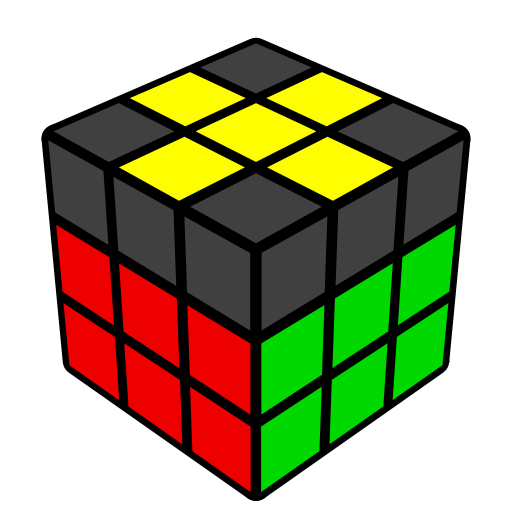
\includegraphics[width=\textwidth]{fakecross.png}
		\caption{Incomplete cross}\label{fig:fakecross}
	\end{subfigure}
	\begin{subfigure}[b]{0.3\textwidth}
		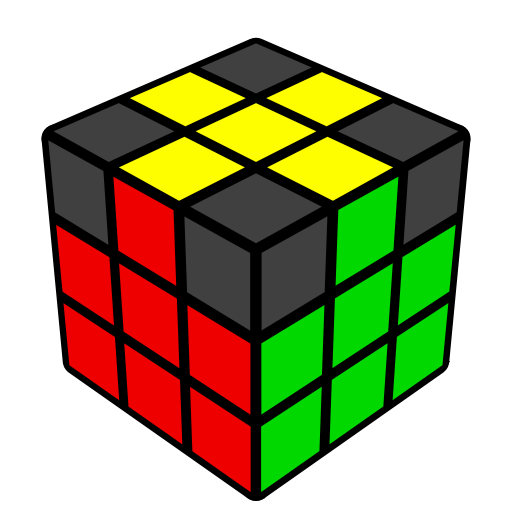
\includegraphics[width=\textwidth]{realcross.png}
		\caption{`Fixed' cross}\label{fig:realcross}
	\end{subfigure}
	\caption{Bottom cross}
\end{figure}


\subsection{Final Layer}